\documentclass[11pt]{article}

% --- Geometry & Layout ---
\usepackage[a4paper, margin=0.5in, top=0.5in, bottom=0.6in]{geometry}
\usepackage{setspace}
\usepackage{fancyhdr}
\usepackage{lastpage}

% --- Typography & Math ---
\usepackage[T1]{fontenc}
\usepackage{mathpazo} % Palatino font
\usepackage{amsmath, amssymb, amsthm}
\usepackage{mathtools}
\usepackage{array, booktabs}
\usepackage{caption} 

% --- Graphics & Colors ---
\usepackage[table, svgnames]{xcolor}
\usepackage{graphicx}
\usepackage{tikz}
\usetikzlibrary{arrows.meta, positioning, shapes.geometric, calc, backgrounds, patterns}
\usepackage{pgfplots}
\pgfplotsset{compat=1.18}

% --- Boxed Environments ---
\usepackage[most]{tcolorbox}

% Define Colors
\definecolor{primary}{RGB}{0, 85, 145}      
\definecolor{secondary}{RGB}{200, 50, 50}   
\definecolor{boxfill}{RGB}{245, 248, 250}   
\definecolor{compltext}{RGB}{0, 100, 0}     % Dark Green for text
\definecolor{complbg}{RGB}{235, 250, 235}   % Light Green for background

% --- VS Code Light Theme (Clean) Configuration ---
\usepackage{listings}
\tcbuselibrary{listings, skins}

% 1. Define VS Code Light Colors
\definecolor{vsclightback}{RGB}{255, 255, 255}   % White Background
\definecolor{vsclightblue}{RGB}{0, 0, 255}       % Keywords (Blue)
\definecolor{vsclightgreen}{RGB}{0, 128, 0}      % Comments (Green)
\definecolor{vsclightpurple}{RGB}{175, 0, 219}   % Control Flow (Purple)
\definecolor{vsclightred}{RGB}{163, 21, 21}      % Strings (Red)
\definecolor{vsclighttext}{RGB}{0, 0, 0}         % Plain Text (Black)
\definecolor{vsctitlebg}{RGB}{243, 243, 243}     % Light Gray Title Bar
\definecolor{vscborder}{RGB}{204, 204, 204}      % Light Border

% 2. Define the Listing Style
\lstdefinestyle{vslightstyle}{
    language=C++,
    basicstyle=\ttfamily\small\color{vsclighttext},
    backgroundcolor=\color{vsclightback},
    commentstyle=\color{vsclightgreen}\itshape,
    keywordstyle=\color{vsclightblue}\bfseries,
    keywordstyle={[2]\color{vsclightpurple}\bfseries},
    stringstyle=\color{vsclightred},
    numberstyle=\tiny\color{gray},
    numbers=none,
    tabsize=4,
    showspaces=false,
    showstringspaces=false,
    breaklines=true,
    frame=none,
    morekeywords={include, define, endif, ifndef, using, namespace},
    morekeywords=[2]{return, if, else, for, while, switch, case, break}
}

% 3. Create the TColorBox Environment
\newtcblisting{vscode}[2][]{
    enhanced,
    listing only,
    listing engine=listings,
    listing options={style=vslightstyle},
    title={#2},
    coltitle=black,
    fonttitle=\small\ttfamily,
    colback=vsclightback,
    colframe=vscborder,
    sharp corners,
    top=0mm, bottom=0mm,
    colbacktitle=vsctitlebg,
    #1
}

% --- Complexity badge ---
\newcommand{\complexity}[1]{%
  \tcbox[on line, 
    colback=complbg, 
    colframe=compltext!50, 
    boxrule=0.5pt, 
    arc=2pt, 
    boxsep=0pt, 
    left=3pt, right=3pt, top=2pt, bottom=2pt
  ]{\color{compltext}\small\ensuremath{#1}}%
}

% Style for Section Headers
\usepackage{titlesec}
\titleformat{\section}
  {\color{primary}\Large\bfseries}
  {\thesection}{1em}{}[\titlerule]
\titleformat{\subsection}
  {\color{primary}\large\bfseries}
  {\thesubsection}{1em}{}

% Custom Boxes
\newtcolorbox{conceptbox}[2][]{
  enhanced,
  title={#2},
  colframe=primary,
  colback=boxfill,
  coltitle=white,
  fonttitle=\bfseries,
  attach boxed title to top left={xshift=5mm, yshift*=-3mm},
  boxed title style={frame hidden, size=small, rounded corners},
  drop fuzzy shadow,
  #1
}

\newtcolorbox{resultbox}{
  enhanced,
  colframe=secondary,
  colback=red!5!white,
  borderline={0.5mm}{0mm}{secondary},
  boxrule=0.5pt,
  sharp corners,
  fontupper=\bfseries\centering\large
}

\newtcolorbox{derivation}{
  blanker,
  borderline west={1mm}{0pt}{lightgray},
  left=15pt,
  fontupper=\small
}

% --- Math shortcuts ---
\DeclareMathOperator{\lcm}{lcm}
\DeclareMathOperator{\rad}{rad}
\newcommand{\cnt}{\operatorname{cnt}}
\newcommand{\Id}{\operatorname{Id}}

% --- Line Spacing ---
\setstretch{1.18}
\setlength{\parindent}{0pt}
\setlength{\parskip}{8pt}

% --- Header/Footer ---
\pagestyle{fancy}
\fancyhf{}
\fancyfoot[C]{\thepage\ / \pageref{LastPage}}
\renewcommand{\headrulewidth}{0pt}

% hyperref is loaded last on purpose
\usepackage[colorlinks=true, linkcolor=primary, urlcolor=secondary]{hyperref}

% --- Document Start ---
\begin{document}

% --------------------- TITLE PAGE ---------------------
\begin{titlepage}
    \begin{tikzpicture}[remember picture, overlay]
        \fill[primary] (current page.north west) rectangle ($(current page.north east)-(0,2)$);
        \fill[primary] (current page.south west) rectangle ($(current page.south east)+(0,1)$);
        \node[opacity=0.1, anchor=center] at (current page.center) {
            \scalebox{10}{$\sum$}
        };
    \end{tikzpicture}

    \centering
    \vspace*{3cm}

    {\Huge \bfseries \color{primary} Number Theory}\\[0.5cm]
    {\Large \textsc{Summation of Multiplicative Functions}}\\[1cm]

    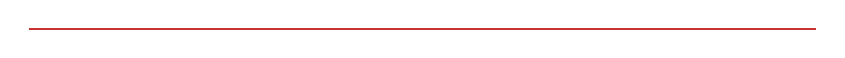
\begin{tikzpicture}
        \draw[thick, secondary] (0,0) -- (10,0);
    \end{tikzpicture}\\[1cm]

    {\large \textbf{Derivations and C++ Implementations}}\\[0.5cm]

    \vfill

    \today
\end{titlepage}

\tableofcontents
\clearpage

% --------------------- CONTENT ---------------------

\section{Notation \& Definitions}
\label{sec:notation}

Before deriving the summations, we define the standard notations and key multiplicative functions used in Number Theory.

\begin{conceptbox}{Standard Notation}
    \begin{itemize}
        \item $[P]$ : \textbf{Iverson Bracket}. Returns $1$ if predicate $P$ is true, $0$ otherwise.
        \item $\lfloor x \rfloor$ : Floor function (integer part).
        \item $d \mid n$ : Integer $d$ divides integer $n$.
    \end{itemize}
\end{conceptbox}

\subsection{Common Multiplicative Functions}
A function $f$ is \textit{multiplicative} if $f(1)=1$ and $f(ab) = f(a)f(b)$ whenever $\gcd(a,b)=1$. Such a function is determined by its values on prime powers $p^k$. Below are the standard examples:

\begin{center}
    \renewcommand{\arraystretch}{1.5}
    \begin{tabular}{l l l}
        \toprule
        \textbf{Function Name}             & \textbf{Symbol} & \textbf{Value at } $p^k$                                   \\
        \midrule
        Constant function                  & $I(p^k)$        & $1$                                                        \\
        Identity function                  & $\Id(p^k)$      & $p^k$                                                      \\
        Unit function                      & $\epsilon(p^k)$ & $[p^k = 1]$                                                \\
        Sum of divisors                    & $\sigma_1(p^k)$ & $\frac{p^{k+1}-1}{p-1}$                                    \\
        Möbius function                    & $\mu(p^k)$      & $\begin{cases} 1 & k=0 \\ -1 & k=1 \\ 0 & k>1 \end{cases}$ \\
        \rowcolor{boxfill} Euler's totient & $\phi(p^k)$     & $p^k - p^{k-1}$ \quad ($k \ge 1$)                          \\
        \bottomrule
    \end{tabular}
\end{center}

\begin{conceptbox}{Lemma: Complexity of Divisor Sums}
    When implementing sums involving divisors (or multiples), a common pattern is to loop $i$ from $1$ to $n$, and for each $i$, loop through its multiples $j = i, 2i, 3i, \dots, n$.

    The total number of iterations is the sum of the count of multiples for each $i$:
    \[ \sum_{i=1}^n \left\lfloor \frac{n}{i} \right\rfloor \le n \sum_{i=1}^n \frac{1}{i} = n H_n \]
    Since the harmonic number $H_n$ grows as $\ln n + O(1)$, the total time complexity is:
    \[ \complexity{O(n \log n)} \]
\end{conceptbox}

\newpage
\section{Fundamental Identity: Sum of Euler's Totient}
\label{sec:proof_identity}

We intend to prove the property that connects divisors to the number itself.

\begin{resultbox}
    \begin{equation}
        \sum_{d \mid n} \phi(d) = n \label{eq:euler_identity}
    \end{equation}
\end{resultbox}

\begin{vscode}{Verify Fundamental Identity for n}
ll sum = 0;
for (const int &d : divs)
    sum += phi[d];
// sum will always equal n
\end{vscode}

\textbf{Proof strategy:} If $f$ is multiplicative, then so is $F(n)=\sum_{d\mid n} f(d)$ (every divisor of $ab$ with $\gcd(a,b)=1$ factors uniquely as $d_1 d_2$ with $d_1\mid a$, $d_2\mid b$). Since $\phi$ is multiplicative, $F$ is multiplicative, and the identity $F(n)=n$ also holds for the multiplicative function $n\mapsto n$. It therefore suffices to check it on prime powers $n=p^k$.

\begin{derivation}
    The divisors of $p^k$ are $\{1, p, p^2, \dots, p^k\}$. The sum becomes:
    \begin{align*}
        \sum_{d \mid p^k} \phi(d) & = \sum_{j=0}^k \phi(p^j)                            \\
                                  & = \phi(1) + \phi(p) + \phi(p^2) + \dots + \phi(p^k)
    \end{align*}
    Substituting $\phi(p^j) = p^j - p^{j-1}$ (for $j \ge 1$) and $\phi(1)=1$, the sum telescopes:
    \begin{align*}
        1 + (p-1) + (p^2-p) + \dots + (p^k-p^{k-1}) = p^k.
    \end{align*}
\end{derivation}

\vspace{0.5cm}

% --- TIKZ TELESCOPING VISUALIZATION ---
\begin{center}
    \captionsetup{hypcap=false}
    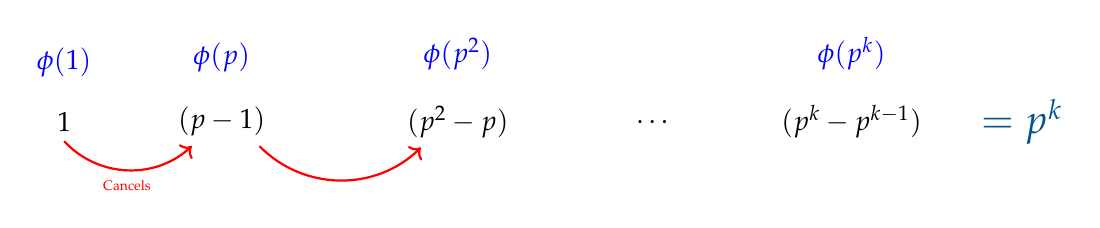
\begin{tikzpicture}[node distance=1.5cm]
        \node (t0) at (0,0) {$1$};
        \node (t1) at (2,0) {$(p - 1)$};
        \node (t2) at (5,0) {$(p^2 - p)$};
        \node (dots) at (7.5,0) {$\dots$};
        \node (tk) at (10,0) {$(p^k - p^{k-1})$};

        % Arrows canceling terms
        \draw[->, red, thick, bend right=45] (t0.south) to node[below, font=\tiny] {Cancels} ($(t1.south west)+(0.3,0)$);
        \draw[->, red, thick, bend right=45] ($(t1.south east)+(-0.2,0)$) to ($(t2.south west)+(0.3,0)$);

        \node[above=0.2cm of t0, blue] {$\phi(1)$};
        \node[above=0.2cm of t1, blue] {$\phi(p)$};
        \node[above=0.2cm of t2, blue] {$\phi(p^2)$};
        \node[above=0.2cm of tk, blue] {$\phi(p^k)$};

        % Result
        \node[right=0.5cm of tk, font=\bfseries\Large, color=primary] {$= p^k$};
    \end{tikzpicture}
    \captionof{figure}{Visualizing the Telescoping Sum}
\end{center}

Since the sum equals $p^k = n$ for every prime power, and both sides are multiplicative in $n$, the identity holds for all positive integers $n$.

\pagebreak
\section{Single Summation (Pillai's Function)}
\label{sec:pillai}

We consider the summation where $n$ is fixed. This is known as \textbf{Pillai's arithmetical function}.

\[ S = \sum_{i=1}^n \gcd(i, n) \]

\subsection{Grouping by GCD Value}
Instead of summing sequentially from $1$ to $n$, we group the terms based on the value of their GCD. Let $d$ be a divisor of $n$. We ask: \textbf{How many times does the value $d$ appear in the sum?}

\begin{derivation}
    The value $d$ appears whenever $\gcd(i, n) = d$. This forces $d \mid i$, so write $i = dk$ with $1 \le k \le n/d$:
    \begin{align*}
        \gcd(dk, n) = d & \iff \gcd(k, n/d) = 1.
    \end{align*}
    The number of integers $k \in [1, n/d]$ coprime to $n/d$ is exactly $\phi(n/d)$.
    Therefore, the value $d$ contributes $d \times \phi(n/d)$ to the total sum.
\end{derivation}

\begin{resultbox}
    \begin{equation}
        \sum_{i=1}^n \gcd(i, n) = \sum_{d \mid n} d \cdot \phi\left(\frac{n}{d}\right) \label{eq:pillai_result}
    \end{equation}
\end{resultbox}

\begin{vscode}{Pillai's Function from the Divisors of $n$}
ll sum = 0;
for (const int &d : divs[n])
    sum += 1LL * d * phi[n / d];
\end{vscode}

\subsection{Example: n = 12}
For $n=12$ the divisors are $\{1, 2, 3, 4, 6, 12\}$ and the formula is $\sum_{d\mid 12} d \cdot \phi(12/d)$:

\begin{center}
    \rowcolors{2}{white}{boxfill}
    \begin{tabular}{c c c c}
        \toprule
        \textbf{Divisor} $d$                & \textbf{Ratio} $n/d$ & \textbf{Count} $\phi(n/d)$ & \textbf{Contribution} \\
        \midrule
        1                                   & 12                   & $\phi(12)=4$               & $1 \times 4 = 4$      \\
        2                                   & 6                    & $\phi(6)=2$                & $2 \times 2 = 4$      \\
        3                                   & 4                    & $\phi(4)=2$                & $3 \times 2 = 6$      \\
        4                                   & 3                    & $\phi(3)=2$                & $4 \times 2 = 8$      \\
        6                                   & 2                    & $\phi(2)=1$                & $6 \times 1 = 6$      \\
        12                                  & 1                    & $\phi(1)=1$                & $12 \times 1 = 12$    \\
        \midrule
        \multicolumn{3}{r}{\textbf{Total:}} & \textbf{40}                                                               \\
        \bottomrule
    \end{tabular}
\end{center}

\pagebreak
\section{Efficient Computation of Pillai's Function}
\label{sec:pillai_optimization}

We previously established that the sum of GCDs (Pillai's function) is given by:
\[ P(n) = \sum_{i=1}^n \gcd(i, n) = \sum_{d \mid n} d \cdot \phi\left(\frac{n}{d}\right) \]
Since a totient table up to $n$ is impractical for large $n$, we exploit the multiplicativity of $P$ instead.

\subsection{Closed Form for Prime Powers}

Since $P = f * g$ is the Dirichlet convolution of $f(n) = n$ and $g(n) = \phi(n)$ (both multiplicative), and the convolution of multiplicative functions is multiplicative, $P$ is multiplicative. This means if $n = p_1^{e_1} \dots p_k^{e_k}$, then $P(n) = \prod P(p_i^{e_i})$.

We derive the value of $P(p^e)$ for a prime power:

\begin{derivation}
    Let $n = p^e$. The divisors are $p^0, p^1, \dots, p^e$.
    \[ P(p^e) = \sum_{r=0}^e p^r \phi(p^{e-r}) \]
    Separating the last term ($r=e$) where $\phi(p^0) = \phi(1) = 1$:
    \[ = \sum_{r=0}^{e-1} p^r \phi(p^{e-r}) + p^e \]
    Using $\phi(p^k) = p^k - p^{k-1}$:
    \[ {}= \sum_{r=0}^{e-1} p^r (p^{e-r} - p^{e-r-1}) + p^e
        \;\overset{\scriptstyle p^r p^{e-r} = p^e}{=}\;
        \textcolor{secondary}{\sum_{r=0}^{e-1} (p^e - p^{e-1})} + p^e \]
    The term inside the sum is constant with respect to $r$. There are $e$ terms (from $0$ to $e-1$).
    \[ {}= e(p^e - p^{e-1}) + p^e
        \;\overset{\scriptstyle \text{distribute } e}{=}\;
        \textcolor{secondary}{e p^e - e p^{e-1}} + p^e \]
    Grouping $p^e$ terms:
\end{derivation}

\begin{resultbox}
    \begin{equation}
        P(p^e) = (e+1)p^e - e p^{e-1}
        \label{eq:pillai_prime_power}
    \end{equation}
    \begin{equation}
        P(n) = \prod_{i=1}^k \left( (e_i+1)p_i^{e_i} - e_i p_i^{e_i-1} \right)
        \label{eq:pillai_prime_power_for_n}
    \end{equation}
\end{resultbox}

\begin{vscode}{P(n) using Prime Factorization Closed Form}
ll res = 1;
for (const auto &[p, e] : mp)
{
    ll pPow = 1;
    for (int i = 0; i < e; i++) pPow *= p;
    res *= (e + 1) * pPow - e * (pPow / p);
}
\end{vscode}

\section{Derivation of Double GCD Summation}
\label{sec:double_gcd}

We now extend this to compute the sum of GCDs for all pairs up to $n$:
\[ \sum_{i=1}^n \sum_{j=1}^n \gcd(i, j) \]

\subsection{The ``Divisor Switching'' Technique}

\begin{derivation}

    Using the identity $\sum_{d \mid x} \phi(d) = x$, we substitute $x$ with $\gcd(i, j)$:

    \[ \sum_{i=1}^n \sum_{j=1}^n \underbrace{\sum_{d \mid \gcd(i, j)} \phi(d)}_{=\gcd(i,j)} \]

    The condition $d \mid \gcd(i, j)$ is equivalent to $(d \mid i) \land (d \mid j)$:
    \[ \sum_{i=1}^n \sum_{j=1}^n \sum_{d = 1}^n \phi(d) [d \mid i][d \mid j]\]
    We swap the summation order to iterate over $d$ first.
    \[ \sum_{d=1}^n \phi(d) \sum_{i = 1}^n [d \mid i] \sum_{j = 1}^n [d \mid j] \]

    For a fixed $d$, how many $i \in [1, n]$ are multiples of $d$? Exactly $\lfloor \frac{n}{d} \rfloor$.
    Similarly for $j$, there are $\lfloor \frac{n}{d} \rfloor$ multiples.
    Thus, the term $\phi(d)$ appears $\lfloor \frac{n}{d} \rfloor \times \lfloor \frac{n}{d} \rfloor$ times.
\end{derivation}

\begin{resultbox}
    \begin{equation}
        \sum_{i=1}^n \sum_{j=1}^n \gcd(i, j) = \sum_{d=1}^n \phi(d) \left\lfloor \frac{n}{d} \right\rfloor^2 \label{eq:double_gcd_result}
    \end{equation}
\end{resultbox}

\begin{vscode}{Double GCD Summation (given phi[], O(n))}
ll sum = 0;
for (int d = 1; d <= n; d++)
{
    ll cnt = n / d;
    sum += phi[d] * cnt * cnt;
}
\end{vscode}
\pagebreak
\section{Summation over Distinct Pairs \texorpdfstring{($i < j$)}{(i < j)}}
\label{sec:upper_triangular_gcd}

We now wish to calculate the sum of GCDs for strict pairs, avoiding the diagonal and duplicates:
\[ S_{upper} = \sum_{i=1}^{n-1} \sum_{j=i+1}^n \gcd(i, j) \]

\subsection{Symmetry Argument}

\begin{derivation}
    Consider the sum over the entire square $1 \le i, j \le n$, namely
$S_{total} = \sum_{i=1}^n \sum_{j=1}^n \gcd(i,j)$ from Section \ref{sec:double_gcd}. \\We can break this total sum into three parts:
    \begin{enumerate}
        \item The diagonal where $i = j \implies \sum_{i=1}^n \gcd(i,i) = \sum_{i=1}^n i = \frac{n(n+1)}{2}$.
        \item The lower triangle where $j < i\implies \sum_{j=1}^{i-1} \gcd(i,j)$.
        \item The upper triangle where $i < j\implies \sum_{j=i+1}^n \gcd(i,j)$.
    \end{enumerate}

    Since $\gcd(i, j) = \gcd(j, i)$, the sum over the lower triangle is identical to the sum over the upper triangle, so $S_{upper} = S_{lower}$. We calculate the lower triangle instead.
    \[ S_{lower} = \sum_{i=1}^n \sum_{j=1}^{i-1} \gcd(i,j) \]
    To be able to apply \hyperref[eq:pillai_result]{Pillai's equation}, we rewrite it in the form
    \[ S_{lower} = \sum_{i=1}^n \sum_{j=1}^{i} \gcd(i,j) - \underbrace{\sum_{i=1}^n \gcd(i,i)}_{n(n+1)/2} \]
\end{derivation}

\begin{resultbox}
    \begin{equation}
        S_{upper} = S_{lower} = \sum_{i=1}^n \sum_{d \mid i} d \cdot \phi\!\left(\frac{i}{d}\right) - \frac{n(n+1)}{2}
        \label{eq:strict_gcd_result}
    \end{equation}
\end{resultbox}

\begin{vscode}{O(n log n) Precomputing using Harmonic Series}
vector<ll> res(n + 1, 0);
for (int i = 1; i <= n; i++)
{
    for (int j = i; j <= n; j += i)
        res[j] += 1LL * i * phi[j / i];
    res[i] -= i;
}
for (int i = 1; i <= n; i++)
    res[i] += res[i - 1];
\end{vscode}

We can optimize this to \complexity{O(n)} by recognizing that the inner sum $\sum_{d \mid i} d \cdot \phi(i/d)$ is exactly Pillai's function $P(i)$. Since $P(i)$ is a multiplicative function, we can precompute it for all values up to $n$ using a \textbf{Linear Sieve}.
The required answer is then just the prefix sums of $P(i) - i$.

\begin{vscode}{O(n) Precomputing using Linear Sieve}
vector<int> primes, low; // low[i] = largest power of lpf(i) dividing i
vector<ll> pillai;
void precomputePillai(int n) 
{
    low.assign(n + 1, 0); pillai.assign(n + 1, 0); pillai[1] = 1;
    for (int i = 2; i <= n; i++) 
    {
        if (!low[i]) low[i] = i, pillai[i] = 2LL * i - 1, primes.push_back(i);
        for (int p : primes) 
        {
            if (1LL * i * p > n) break;
            int m = i * p;
            if (i % p) 
                low[m] = p, pillai[m] = pillai[i] * pillai[p];
            else 
            {
                low[m] = low[i] * p;
                pillai[m] = low[m] == m ? pillai[i] * p + m - i
                                        : pillai[m / low[m]] * pillai[low[m]];
                break;
            }
        }
    }
}
// then: res[i] = res[i-1] + pillai[i] - i
\end{vscode}

\pagebreak
\section{Counting Pairs with Fixed GCD}
\label{sec:fixed_gcd_pairs}

We now consider the problem of counting pairs $(i, j)$ such that $i \le j$ and their greatest common divisor is exactly a specific value $d \ge 1$.

\[ S = \sum_{i=1}^n \sum_{j=i}^n [\gcd(i, j) = d] \]

\subsection{Reduction to Euler's Totient}

\begin{derivation}
    To satisfy the condition $\gcd(i, j) = d$, both $i$ and $j$ must be multiples of $d$. We introduce the substitution $i = d \cdot a$ and $j = d \cdot b$. The GCD condition simplifies as follows:
    \[ \gcd(i, j) = d \iff \gcd(d \cdot a, d \cdot b) = d \iff d \cdot \gcd(a, b) = d \]

    Dividing both sides by $d$, the condition reduces to checking for coprime pairs:
    \[ \gcd(a, b) = 1 \]

    Next, we transform the summation bounds. The original constraint $1 \le i \le j \le n$ scales down by a factor of $d$:
    \[ 1 \le a \le b \le \left\lfloor \frac{n}{d} \right\rfloor \]

    We can now rewrite the sum by iterating over $b$ (the larger number) and counting the valid $a$'s (the smaller number). For a fixed $b$, the number of $a \in [1, b]$ with $\gcd(a,b)=1$ is, by definition, Euler's totient $\phi(b)$ (for $b=1$ the only choice is $a=1$, and $\phi(1)=1$):
    \begin{align*}
        S & = \sum_{b=1}^{\lfloor n/d \rfloor} \sum_{a=1}^{b} [\gcd(a, b) = 1] \\
          & = \sum_{b=1}^{\lfloor n/d \rfloor} \phi(b)
    \end{align*}
\end{derivation}

\begin{resultbox}
    \begin{equation}
        \sum_{i=1}^n \sum_{j=i}^n [\gcd(i, j) = d] = \sum_{k=1}^{\lfloor n/d \rfloor} \phi(k)
        \label{eq:fixed_gcd_result}
    \end{equation}
\end{resultbox}

\begin{vscode}{O(1) Queries with Prefix Sums}
// Precomputation
vector<ll> prefPhi(n + 1, 0);
for (int i = 1; i <= n; i++)
    prefPhi[i] = prefPhi[i - 1] + phi[i];

// Query for fixed GCD = d
cout << prefPhi[n / d] << '\n';
\end{vscode}

\pagebreak
\section{Counting Co-prime Pairs}
\label{sec:coprime_pairs}

We wish to find the total number of ordered pairs of integers $(x, y)$ such that $1 \le x, y \le n$ and $\gcd(x, y) = 1$.
\[ S = \sum_{x=1}^n \sum_{y=1}^n [\gcd(x, y) = 1] \]

\subsection{Derivation via Symmetry}

\begin{derivation}
    We split the summation into three distinct regions based on the relationship between $x$ and $y$:
    \[ S = \underbrace{\sum_{x < y} [\gcd(x, y)=1]}_{\text{Upper Triangle}} + \underbrace{\sum_{x = y} [\gcd(x, y)=1]}_{\text{Diagonal}} + \underbrace{\sum_{x > y} [\gcd(x, y)=1]}_{\text{Lower Triangle}} \]

    \textbf{1. The Diagonal ($x = y$):} \\
    The condition becomes $\gcd(x, x) = 1$, which implies $x = 1$. Thus, there is exactly \textbf{1} solution on the diagonal: $(1, 1)$.

    \textbf{2. The Triangles ($x < y$):} \\
    Due to the symmetry $\gcd(x, y) = \gcd(y, x)$, the count in the upper triangle equals the count in the lower triangle.
    For a fixed $y$, we need to count $x < y$ such that $\gcd(x, y) = 1$. By definition, for $y > 1$, this count is exactly Euler's Totient function $\phi(y)$.
    \[ \sum_{1 \le x < y \le n} [\gcd(x, y) = 1] = \sum_{i=2}^n \phi(i) \]

    \textbf{Total Sum:} \\
    Combining these parts:
    \begin{align*}
        S & = 1 + 2 \sum_{i=2}^n \phi(i)                                                    \\
          & = 2\phi(1) - 1 + 2 \sum_{i=2}^n \phi(i) \quad \text{(since } \phi(1)=1 \text{)} \\
          & = 2 \sum_{i=1}^n \phi(i) - 1
    \end{align*}
\end{derivation}

\begin{resultbox}
    \begin{equation}
        S_n = 2 \sum_{i=1}^n \phi(i) - 1
        \label{eq:coprime_count}
    \end{equation}
\end{resultbox}

\begin{vscode}{Count Co-prime pairs up to n}
// Assumes prefPhi is precomputed
cout << 2 * prefPhi[n] - 1 << '\n';
\end{vscode}

\textbf{Note:} If we wanted unordered pairs where $1 \le i \le j \le n$, the answer would simply be the sum of $\phi$ (i.e., \texttt{prefPhi[n]}).

\pagebreak
\section{Counting Co-prime Sequences (Paths)}
\label{sec:coprime_sequences}

We wish to find the number of sequences of length $N$ where each element $A_i$ is between $1$ and $M$, and adjacent elements are relatively prime ($\gcd(A_i, A_{i+1}) = 1$ for all $1 \le i < N$).

This can be solved efficiently depending on the constraints of $N$ and $M$:
\begin{itemize}
    \item \textbf{Matrix Exponentiation} for small $M$ (e.g., $100$) and large $N$ (e.g., $10^8$).
    \item \textbf{Möbius Inversion DP} for large $M$ (e.g., $10^5$) and small $N$ (e.g., $10^2$).
\end{itemize}

\subsection{Matrix Exponentiation (Large \texorpdfstring{$N$}{N}, Small \texorpdfstring{$M$}{M})}

\begin{derivation}
    We model this as finding paths of length $N-1$ in a graph.
    Each integer from $1$ to $M$ is a vertex. A directed edge exists from $i$ to $j$ if $\gcd(i, j) = 1$.
    The adjacency matrix $A$ is defined as $A_{i,j} = [\gcd(i, j) = 1]$.
    Raising this matrix to the $(N-1)$-th power yields a matrix where the entry at $(i, j)$ is the number of valid lists of length $N$ starting at $i$ and ending at $j$. The total number of valid lists is the sum of all elements in $A^{N-1}$.
    This approach runs in \complexity{O(M^3 \log N)}.
\end{derivation}

\begin{vscode}{Matrix Exponentiation ($O(M^3 \log N)$)}
// A^0 is the identity, so N = 1 correctly returns M
ll n, m;
cin >> n >> m;
TransMatrix mat; // Custom struct for square matrix
for (int i = 1; i <= m; i++)
{
    for (int j = 1; j <= m; j++)
    {
        if (gcd(i, j) == 1)
            mat[i][j] = 1;
    }
}
auto res = mat.matrixPower(n - 1);
Mint ans{};
for (int i = 1; i <= m; i++)
{
    for (int j = 1; j <= m; j++)
        ans += res[i][j];
}
cout << ans << '\n';
\end{vscode}

\subsection{Möbius Inversion DP (Large \texorpdfstring{$M$}{M}, Small \texorpdfstring{$N$}{N})}

\begin{derivation}
    Let $f(k, x)$ be the number of valid sequences of length $k$ ending in $x$.
    The naive transition is:
    \[ f(k, x) = \sum_{y=1}^M [\gcd(x, y) = 1] f(k-1, y) \]
    Applying Möbius Inversion to the condition: $[\gcd(x, y) = 1] = \sum_{d \mid \gcd(x, y)} \mu(d)$.
    \begin{align*}
        f(k, x) & = \sum_{y=1}^M \sum_{\substack{d \mid x \\ d \mid y}} \mu(d) f(k-1, y)      \\
                & = \sum_{d \mid x} \mu(d) \sum_{c=1}^{\lfloor M/d \rfloor} f(k-1, c \cdot d)
    \end{align*}
    We define an auxiliary sum $S(k-1, d)$ representing the sum of $f$ over all multiples of $d$:
    \[ S(k-1, d) = \sum_{c=1}^{\lfloor M/d \rfloor} f(k-1, c \cdot d) \]
    This reduces the transition to two \complexity{O(M \log M)} steps:
    \begin{enumerate}
        \item Compute $S(k-1, d)$ for all $d$.
        \item Compute $f(k, x) = \sum_{d \mid x} \mu(d) S(k-1, d)$ for all $x$.
    \end{enumerate}
    The total complexity to find all paths of length $N$ is \complexity{O(N \cdot M \log M)}.
\end{derivation}

\begin{vscode}{Möbius Inversion DP ($O(N \cdot M \log M)$)}
vector<Mint> f(m + 1, Mint(1)); // Base case: length 1 (f[0] is unused)
vector<Mint> S(m + 1, Mint(0));

for (int step = 2; step <= n; step++)
{
    // Compute S(d) = sum of f for multiples of d
    fill(S.begin(), S.end(), Mint(0));
    for (int d = 1; d <= m; d++)
    {
        for (int c = d; c <= m; c += d)
            S[d] += f[c];
    }
    fill(f.begin(), f.end(), Mint(0));
    for (int d = 1; d <= m; d++)
    {
        if (mu[d] == 0) continue;
        for (int x = d; x <= m; x += d)
        {
            if (mu[d] == 1) f[x] += S[d];
            else f[x] -= S[d];
        }
    }
}
Mint ans = 0;
for (int i = 1; i <= m; i++) ans += f[i];
\end{vscode}

\pagebreak
\section{Sum of Numbers with Fixed GCD}
\label{sec:sum_fixed_gcd}

We want to find the sum of all integers $1 \le i < n$ whose greatest common divisor with $n$ is exactly $d$, where $d \mid n$ and $d < n$ (if $d \nmid n$ the sum is empty, and if $d = n$ there is no valid $i$).
\[ S = \sum_{1 \le i < n} i \cdot [\gcd(i, n) = d] \]

\subsection{Derivation}

\begin{derivation}
    First, we note that if $\gcd(i, n) = d$, then $d$ must divide $i$. We substitute $i = d \cdot k$. The condition $1 \le i < n$ implies $1 \le k < \frac{n}{d}$.
    \[ S = \sum_{1 \le k < n/d} (d \cdot k) \cdot [\gcd(dk, n) = d] \]

    Simplifying the GCD condition: $\gcd(dk, n) = d \iff \gcd(k, n/d) = 1$.
    Let $m = \frac{n}{d}$. The sum becomes:
    \[ S = d \sum_{1 \le k < m} k \cdot [\gcd(k, m) = 1] \]

    We now calculate the inner sum, which is the sum of integers coprime to $m$ in the range $[1, m)$.
    Here $m = n/d > 1$. We use the symmetry $\gcd(k, m) = 1 \iff \gcd(m-k, m) = 1$, so $k \mapsto m-k$ is a bijection on the set $C$ of integers in $[1,m)$ coprime to $m$. Hence
    \[ \sum_{k \in C} k = \sum_{k \in C} (m-k) \implies 2\sum_{k \in C} k = \sum_{k \in C} m = m\,\phi(m), \]
    that is,
    \[ \sum_{1 \le k < m} k \cdot [\gcd(k, m) = 1] = \frac{m \cdot \phi(m)}{2}. \]
\end{derivation}

\begin{resultbox}
    Substituting back $m = n/d$:
    \begin{equation}
        \sum_{1 \le i < n} i \cdot [\gcd(i, n) = d] = \frac{n \cdot \phi(n/d)}{2}
        \label{eq:sum_gcd_d}
    \end{equation}
\end{resultbox}

\begin{vscode}{Sum of numbers with GCD = d}
// assumes d divides n
if (d == n)
    cout << 0 << '\n';
else
    cout << 1LL * n * phi[n / d] / 2 << '\n';
\end{vscode}

\begin{conceptbox}{Corollary: Sum of Coprimes}
    A very common case is determining the sum of integers less than $n$ that are relatively prime to $n$. By setting $d=1$ in Eq.~\eqref{eq:sum_gcd_d}:
    \begin{equation}
        \sum_{\substack{1 \le k < n \\ \gcd(k, n) = 1}} k = \frac{n \cdot \phi(n)}{2} \quad \text{for } n > 1
    \end{equation}
\end{conceptbox}

\pagebreak
\section{LCM Summations}
\label{sec:lcm_summation}

Sums involving the least common multiple rely on the identity $\lcm(i, n) = \dfrac{i \cdot n}{\gcd(i, n)}$.

\subsection{Sum of \texorpdfstring{$\operatorname{lcm}(i, n)$}{lcm(i, n)}}

\begin{conceptbox}{Goal}
    Compute $S = \sum_{i=1}^n \lcm(i, n)$.
\end{conceptbox}

\textbf{Step 1: Isolate the last term.}
We separate the term for $i=n$ (where $\lcm(n, n) = n$) to make the summation symmetric.
\[ S - n = \sum_{i=1}^{n-1} \lcm(i, n) \quad \dots (1) \]

\textbf{Step 2: Reverse and Add.}
We write the sum in reverse order. Note that $\lcm(i, n)$ runs over the same values as $\lcm(n-i, n)$.
\[ S - n = \sum_{i=1}^{n-1} \lcm(n-i, n) \quad \dots (2) \]
Adding equations (1) and (2):
\[ 2(S - n) = \sum_{i=1}^{n-1} \left( \lcm(i, n) + \lcm(n-i, n) \right) \]

\textbf{Step 3: Simplify the pair sum.}
Using the definition of LCM and the property $\gcd(n-i, n) = \gcd(i, n)$:
\begin{align*}
    \lcm(i, n) + \lcm(n-i, n) & = \frac{i \cdot n}{\gcd(i, n)} + \frac{(n-i) \cdot n}{\gcd(n-i, n)}     \\
                              & = \frac{i \cdot n + (n-i) \cdot n}{\gcd(i, n)} = \frac{n^2}{\gcd(i, n)}
\end{align*}
Substituting this back into the sum:
\[ 2(S - n) = \sum_{i=1}^{n-1} \frac{n^2}{\gcd(i, n)} = n \sum_{i=1}^{n-1} \frac{n}{\gcd(i, n)} \]

\textbf{Step 4: Group by GCD divisors.}
The term $\frac{n}{d}$ appears whenever $\gcd(i, n) = d$. The number of such $i$ is $\phi(n/d)$.
We sum over divisors $d$ of $n$ (excluding $d=n$ because the sum runs to $n-1$).
\[ 2(S - n) = n \sum_{\substack{d \mid n \\ d \neq n}} \frac{n}{d} \cdot \phi\left(\frac{n}{d}\right) \]
Let $k = n/d$. As $d$ iterates divisors of $n$, $k$ also iterates divisors of $n$ (excluding $k=1$).
\[ 2(S - n) = n \sum_{\substack{k \mid n \\ k \neq 1}} k \cdot \phi(k) \]
We can include $k=1$ (where term is $1 \cdot \phi(1) = 1$) by subtracting it back:
\[ 2(S - n) = n \left( \sum_{k \mid n} (k \cdot \phi(k)) - 1 \right) \]

\begin{resultbox}
    \begin{equation}
        \sum_{i=1}^n \lcm(i, n) = \frac{n}{2} \left( \sum_{d \mid n} (d \cdot \phi(d)) + 1 \right) \label{eq:lcm_result}
    \end{equation}
\end{resultbox}

\begin{vscode}{Precomputing $\sum_{d \mid x} d\phi(d)$ for all $x \le n$}
vector<long long> res(n + 1, 0);
for (int i = 1; i <= n; i++)
{
    for (int j = i; j <= n; j += i)
        res[j] += 1LL * i * phi[i];
}
// x * (res[x] + 1) can overflow 64 bits for large x; reduce modulo a prime or use __int128
cout << 1LL * x * (res[x] + 1) / 2;
\end{vscode}

\subsection{Double Summation of LCM}

We aim to find $\sum_{i=1}^n \sum_{j=1}^n \lcm(i, j)$.
We iterate over all possible values of $g = \gcd(i, j)$.

\begin{enumerate}
    \item \textbf{Rewrite LCM:} $\lcm(i, j) = \frac{i \cdot j}{g}$.
    \item \textbf{Parametrize:} Let $i = g \cdot a$ and $j = g \cdot b$ where $\gcd(a, b) = 1$.
    \item \textbf{New Limits:} If $i, j \le n$, then $a, b \le \lfloor n/g \rfloor$.
\end{enumerate}

\[ \sum_{g=1}^n \frac{1}{g} \sum_{a=1}^{\lfloor n/g \rfloor} \sum_{b=1}^{\lfloor n/g \rfloor} [\gcd(a, b) = 1] (ga)(gb) \]

Pulling out $g^2$ and cancelling one factor of $g$:

\begin{resultbox}
    \begin{equation}
        \sum_{i=1}^n \sum_{j=1}^n \lcm(i, j) = \sum_{g=1}^n g \sum_{a=1}^{\lfloor n/g \rfloor} \sum_{b=1}^{\lfloor n/g \rfloor} [\gcd(a, b) = 1] a \cdot b \label{eq:double_lcm_result}
    \end{equation}
\end{resultbox}

\begin{derivation}
    Put $N_g = \lfloor n/g \rfloor$ and $T(x) = x(x+1)/2$. Replacing $[\gcd(a,b)=1]$ by $\sum_{l \mid \gcd(a,b)} \mu(l)$ and writing $a = la'$, $b = lb'$:
    \[ \sum_{a,b \le N_g} [\gcd(a,b)=1]\, ab = \sum_{l=1}^{N_g} \mu(l)\, l^2\, T\!\left(\left\lfloor \tfrac{N_g}{l} \right\rfloor\right)^2 . \]
    Let $t = gl$. Since $\lfloor \lfloor n/g \rfloor / l \rfloor = \lfloor n/t \rfloor$ and $g\,l^2 = t\,l$:
    \[ \sum_{i=1}^n \sum_{j=1}^n \lcm(i,j) = \sum_{t=1}^n t \, T\!\left(\left\lfloor \tfrac{n}{t} \right\rfloor\right)^2 \sum_{l \mid t} l\,\mu(l). \]
\end{derivation}

\begin{vscode}{O(n log n) using Möbius Inversion}
// f[t] = sum_{d | t} d * mu[d]   (kept in [0, mod))
vector<ll> f(n + 1, 0);
for (int d = 1; d <= n; d++)
{
    if (mu[d] == 0) continue;
    for (int t = d; t <= n; t += d)
        f[t] = ((f[t] + 1LL * d * mu[d]) % mod + mod) % mod;
}

// getSum(x) returns 1 + 2 + ... + x (mod p)
auto getSum = [&](ll x)
{ return x * (x + 1) / 2 % mod; };

ll ans = 0;
for (int t = 1; t <= n; t++)
{
    ll sumTerms = getSum(n / t);
    sumTerms = sumTerms * sumTerms % mod;
    ans = (ans + 1LL * t * f[t] % mod * sumTerms) % mod;
}
\end{vscode}

\pagebreak
\section{Möbius Inversion}
\label{sec:mobius}

\subsection{Definition \& Properties}

Möbius inversion states that if $g(n) = \sum_{d \mid n} f(d)$ for every positive integer $n$, then:
\[ f(n) = \sum_{d \mid n} \mu(d) g\left(\frac{n}{d}\right) \]
where $\mu(x)$ is the Möbius function.

\begin{conceptbox}{Möbius Function $\mu(n)$}
    The function is multiplicative and satisfies:
    \begin{itemize}
        \item $\mu(1) = 1$
        \item $\mu(p) = -1$ (for any prime $p$)
        \item $\mu(p^k) = 0$ (for any $k \ge 2$)
    \end{itemize}
    Most importantly, it satisfies the identity:
    \[ \sum_{d \mid n} \mu(d) = [n = 1] \]
    This property is often more useful than the definition itself for solving sums.
\end{conceptbox}

\begin{vscode}{Linear Sieve for Möbius Function}
vector<int> mu, primes;
void precomputeMu(int n) 
{
    mu.assign(n + 1, 2); 
    mu[1] = 1;
    for (int i = 2; i <= n; i++) 
    {
        if (mu[i] == 2) 
            mu[i] = -1, primes.push_back(i);
        for (const int &p : primes) 
        {
            if (1LL * i * p > n) break;
            mu[i * p] = i % p ? -mu[i] : 0;
            if (i % p == 0) break;
        }
    }
}
\end{vscode}
\newpage
\section{Prime Factorization \& Counting Tricks}
\label{sec:prime_tricks}

\subsection{Counting Coprimes in a Range}
To count the number of integers $x \le m$ such that $\gcd(x, n) = 1$, we use inclusion-exclusion based on the prime factors of $n$.

\begin{conceptbox}{Radical of $n$}
    Let $\rad(n)$ be the product of the distinct prime factors of $n$.
    \[ n = p_1^{a_1} \dots p_k^{a_k} \implies \rad(n) = p_1 \dots p_k \]
    The summation iterates over divisors of the radical (square-free divisors):
\end{conceptbox}

\begin{resultbox}
    \begin{equation}
        \Phi(n, m) = \sum_{d \mid \rad(n)} \mu(d) \left\lfloor \frac{m}{d} \right\rfloor
    \end{equation}
\end{resultbox}

\begin{vscode}{Count coprimes to n in range [1, m]}
// PF: distinct prime factors of n
ll res = 0;
int k = PF.size();
for (int mask = 0; mask < (1 << k); mask++)
{
    ll mult = 1;
    for (int i = 0; i < k; i++)
        if ((mask >> i) & 1)
            mult *= PF[i];
    if (__builtin_popcount(mask) & 1)
        res -= m / mult;
    else
        res += m / mult;
}
\end{vscode}

\subsection{Distinct Prime Factors \texorpdfstring{$\omega(m)$}{omega(m)}}
The function $\omega(m)$ counts the number of distinct prime factors of $m$. This can be computed efficiently during a Linear Sieve.

\begin{vscode}{Compute $\omega(m)$ using LPF array}
vector<int> omega(n + 1);
for (int i = 2; i <= n; i++)
{
    int q = i / LPF[i];
    omega[i] = omega[q] + (LPF[i] != LPF[q]);
}
\end{vscode}
\pagebreak
\subsection{Splitting into Coprime Factors}
We want to find the number of ordered pairs $(a, b)$ of positive integers such that:
\[ a \cdot b = m \quad \text{and} \quad \gcd(a, b) = 1 \]
Since $a$ and $b$ are coprime, they cannot share any prime factors. Thus, for every prime power $p_i^{e_i}$ in the factorization of $m$, the entire term $p_i^{e_i}$ must belong entirely to either $a$ or $b$.
For each of the $\omega(m)$ distinct prime factors, we have 2 choices (for $m=1$ there is exactly one pair, $(1,1)$).

\begin{resultbox}
    \begin{equation}
        \text{Number of ordered pairs} = 2^{\omega(m)}
    \end{equation}
\end{resultbox}

\begin{vscode}{Number of coprime pairs multiplying to m}
// Assuming omega array is precomputed via LPF
cout << modPow(2LL, 1LL * omega[m], mod) << '\n';
\end{vscode}

\subsection{Numbers where \texorpdfstring{$\phi(x) \mid x$}{phi(x) | x}}
We wish to count the number of integers $x \le n$ such that Euler's Totient divides the number itself:
\[ \phi(x) \mid x \]
Writing $x = \prod p_i^{e_i}$ we have $x/\phi(x) = \prod p_i/(p_i-1)$, which depends only on the set of primes of $x$. This ratio is an integer only when that set is $\emptyset$, $\{2\}$ or $\{2,3\}$. Hence the integers satisfying the condition are exactly:
\[ x = 2^a \cdot 3^b \quad \text{for } a \ge 1, b \ge 0 \quad (\text{and } x=1) \]
To solve this for a given $n$, we simply iterate over powers of 2 and 3:
\[ \text{Count} = 1 + \sum_{a \ge 1} \sum_{b \ge 0} [2^a \cdot 3^b \le n] \]

\begin{vscode}{Count the number of integers $x \le n$ such that $\phi(x) \mid x$}
ll cnt = 1; // x = 1
for (ll p2 = 2; p2 <= n; p2 *= 2)
{
    for (ll x = p2; x <= n; x *= 3)
    {
        cnt++;
        if (x > n / 3)
            break; // avoid overflow
    }
}
\end{vscode}

\pagebreak
\section{Counting Coprime Pairs in an Array}
\label{sec:coprime_harmonic}

\textbf{Problem:} Given an array $A$ of size $N$, find the number of pairs of indices $(i, j)$ such that $1 \le i < j \le N$ and $\gcd(A[i], A[j]) = 1$.
\textit{Constraints:} $N, A[i] \le 10^6$.

\subsection{Derivation}

\begin{derivation}
    We wish to calculate the sum of the indicator function $[\gcd(x, y) = 1]$ over all pairs in the array.
    \[ \text{Ans} = \sum_{i < j} [\gcd(A[i], A[j]) = 1] \]
    Using the fundamental Möbius property $\sum_{d \mid n} \mu(d) = [n=1]$, we substitute $n$ with $\gcd(A[i], A[j])$:
    \[ \text{Ans} = \sum_{i < j} \sum_{d \mid \gcd(A[i], A[j])} \mu(d) \]
    The condition $d \mid \gcd(A[i], A[j])$ implies that $d$ must divide both $A[i]$ and $A[j]$. We change the order of summation to iterate over the divisor $d$ first.
    \[ \text{Ans} = \sum_{d=1}^{\max A} \mu(d) \cdot (\text{count of pairs } (i, j) \text{ such that } d \mid A[i] \land d \mid A[j]) \]

    Let $\cnt[x]$ be the frequency of the value $x$ in array $A$, and $V = \max A$.
    Let $D[d]$ be the number of elements in $A$ that are multiples of $d$.
    \[ D[d] = \sum_{k=1}^{\lfloor V/d \rfloor} \cnt[k \cdot d] \]
    If there are $D[d]$ multiples of $d$, the number of ways to choose a pair from them is $\binom{D[d]}{2}$.
\end{derivation}

\begin{resultbox}
    \begin{equation}
        S = \sum_{d=1}^{\max A} \mu(d) \frac{D[d](D[d]-1)}{2}
    \end{equation}
\end{resultbox}

\begin{vscode}{O(V log V) Coprime Pairs in Array}
vector<ll> D(mx + 1, 0);
for (auto &x : a)
    D[x]++;

// D[i] = number of elements divisible by i
for (int i = 1; i <= mx; i++)
{
    for (int j = 2 * i; j <= mx; j += i)
        D[i] += D[j];
}

ll ans = 0;
for (int d = 1; d <= mx; d++)
{
    if (mu[d] == 0)
        continue;
    ll pairs = D[d] * (D[d] - 1) / 2;
    ans += mu[d] * pairs;
}
cout << ans << '\n';
\end{vscode}



\pagebreak
\section{LCM Sum over an Array}
\label{sec:lcm_array}

\textbf{Problem:} Given an array $A$ of size $N$ with values up to $V$, calculate:
\[ \sum_{i=1}^N \sum_{j=1}^N \lcm(A[i], A[j]) \]
\textit{Constraints:} $N \le 2 \cdot 10^5$, $A[i] \le V = 10^6$.

\subsection{Derivation}

\begin{derivation}
    Let $\cnt[x]$ denote the frequency of the value $x$ in array $A$. We group pairs by their values $a, b$:
    \[ \text{Ans} = \sum_{a=1}^V \sum_{b=1}^V \cnt[a]\,\cnt[b] \frac{a \cdot b}{\gcd(a, b)} \]

    \textbf{Step 1: Group by GCD} \\
    We iterate over $d = \gcd(a, b)$. For $\gcd(a, b) = d$ to hold, both $a$ and $b$ must be multiples of $d$, and $\gcd(a/d, b/d) = 1$.
    \[ \text{Ans} = \sum_{d=1}^V \frac{1}{d} \sum_{\substack{a \le V \\ d \mid a}} \sum_{\substack{b \le V \\ d \mid b}} [\gcd(a/d, b/d) = 1]\, ab\, \cnt[a]\, \cnt[b] \]

    \textbf{Step 2: Möbius Inversion} \\
    We substitute $[\gcd(x, y) = 1]$ with $\sum_{l \mid \gcd(x, y)} \mu(l)$.
    Here $x = a/d$ and $y = b/d$. Thus $l$ must divide both $a/d$ and $b/d$, which implies $dl \mid a$ and $dl \mid b$.
    \[ \text{Ans} = \sum_{d=1}^V \frac{1}{d} \sum_{\substack{a \le V \\ d \mid a}} \sum_{\substack{b \le V \\ d \mid b}} ab\, \cnt[a]\, \cnt[b] \sum_{l \mid \gcd(a/d,\, b/d)} \mu(l) \]

    \textbf{Step 3: Change of Variables (The "T" Substitution)} \\
    Let $T = d \cdot l$. We swap the summation order to iterate over $T$ first.
    The term associated with $T$ involves summing over valid $d, l$ such that $dl = T$.
    Since $d = T/l$, the factor $\frac{1}{d}$ becomes $\frac{l}{T}$.
    The condition $dl \mid a$ simply becomes $T \mid a$.

    \[ \text{Ans} = \sum_{T=1}^V \left( \sum_{l \mid T} \frac{l}{T} \mu(l) \right) \left( \sum_{\substack{a \le V \\ T \mid a}} a \cdot \cnt[a] \right) \left( \sum_{\substack{b \le V \\ T \mid b}} b \cdot \cnt[b] \right) \]

    The sums over $a$ and $b$ are identical. Every such $a$ is a multiple $kT$, so the sum is divisible by $T$. Define
    \[ S(T) = \sum_{k=1}^{\lfloor V/T \rfloor} k \cdot \cnt[kT], \qquad \text{so that} \qquad \sum_{T \mid a} a \cdot \cnt[a] = T \cdot S(T). \]
\end{derivation}

\begin{resultbox}
    \begin{equation}
        \text{Ans} = \sum_{T=1}^V T \cdot h(T) \cdot \big(S(T)\big)^2
    \end{equation}
    where the weighting function $h(T)$ is defined as:
    \[ h(T) = \sum_{l \mid T} l \cdot \mu(l) = \prod_{p \mid T} (1-p) \]
\end{resultbox}

\begin{vscode}{O(V log V) LCM Sum on Array}
// h[t] = sum_{l | t} l * mu[l]; answer = sum_t t * h[t] * S(t)^2
vector<ll> cnt(mx + 1, 0);
for (auto &x : a)
    cnt[x]++;

vector<ll> f(mx + 1, 0); // f = h
for (int l = 1; l <= mx; l++)
{
    if (mu[l] == 0)
        continue;
    for (int t = l; t <= mx; t += l)
        f[t] = ((f[t] + 1LL * l * mu[l]) % mod + mod) % mod;
}

ll ans = 0;
for (int t = 1; t <= mx; t++)
{
    ll sT = 0;
    for (int k = t; k <= mx; k += t)
        sT = (sT + 1LL * (k / t) * cnt[k]) % mod;

    ans = (ans + 1LL * t * f[t] % mod * (sT * sT % mod)) % mod;
}
cout << ans << '\n';
\end{vscode}

\pagebreak
\section{Subsets with a Specific GCD}
\label{sec:subsets_gcd}

A common problem in combinatorial number theory is finding the number of non-empty subsets of an array $A$ (of size $N$) such that the greatest common divisor of the elements in the subset is exactly $k$.

Let $M$ be the maximum element in the array $A$. We define two functions:
\begin{itemize}
    \item $F(k)$: The number of non-empty subsets where the GCD is a \textbf{multiple} of $k$.
    \item $f(k)$: The number of non-empty subsets where the GCD is \textbf{exactly} $k$.
\end{itemize}

\subsection{Direct Inclusion-Exclusion (Working Backwards)}

\begin{derivation}
    To compute $F(k)$, we only care about elements in $A$ that are multiples of $k$.
    Let $D[k]$ be the number of elements of $A$ that are multiples of $k$.
    Since we can include or exclude any of these elements (but must pick at least one), the number of such subsets is:
    \[ F(k) = 2^{D[k]} - 1 \]

    The subsets counted in $F(k)$ will have a GCD of $k, 2k, 3k, \dots$. Thus, $F(k)$ is the sum of $f$ over all multiples of $k$:
    \[ F(k) = \sum_{m=1}^{\lfloor M/k \rfloor} f(m \cdot k) \]

    To isolate $f(k)$, we rearrange the formula to subtract the exact counts of all strict multiples of $k$. If we compute this from $M$ down to $1$, $f(m \cdot k)$ will always be known by the time we need to compute $f(k)$.
\end{derivation}

\begin{resultbox}
    \begin{equation}
        f(k) = (2^{D[k]} - 1) - \sum_{m=2}^{\lfloor M/k \rfloor} f(m \cdot k)
    \end{equation}
\end{resultbox}

\begin{vscode}{Count subsets with exactly GCD = k}
vector<ll> cnt(mx + 1, 0), f(mx + 1, 0);
for (auto &x : a)
    cnt[x]++;

for (int i = mx; i >= 1; i--)
{
    ll D = cnt[i], sub = 0; // D = number of elements divisible by i
    for (int j = 2 * i; j <= mx; j += i)
    {
        D += cnt[j];
        sub = (sub + f[j]) % mod;
    }
    f[i] = ((modPow(2LL, D, mod) - 1 - sub) % mod + mod) % mod;
}
/* O(M log M) */
\end{vscode}

\subsection{Formalization via Möbius Inversion (Dual Form)}

While the backward loop is efficient (\complexity{O(M \log M)}) for calculating all $f(k)$, what if we only want $f(1)$ or want an explicit formula without recursive subtraction? We can use the \textbf{Dual Form} of Möbius Inversion.

\begin{conceptbox}{Möbius Inversion over Multiples}
    Standard Möbius inversion operates on divisors:
    \[ G(n) = \sum_{d \mid n} g(d) \implies g(n) = \sum_{d \mid n} \mu(d) G\left(\frac{n}{d}\right) \]
    The \textbf{Dual Form} operates on multiples. If a function is defined as a sum over multiples:
    \[ F(n) = \sum_{m=1}^{\infty} f(m \cdot n) \implies f(n) = \sum_{m=1}^{\infty} \mu(m) F(m \cdot n) \]
\end{conceptbox}

\begin{derivation}
    Applying the dual form to our subset problem where $F(k) = 2^{D[k]} - 1$:
    \[ f(k) = \sum_{m=1}^{\lfloor M/k \rfloor} \mu(m) F(m \cdot k) \]
    This gives us a direct formula for the number of subsets with GCD exactly $k$, independently of other $f$ values.
\end{derivation}

\begin{resultbox}
    \begin{equation}
        f(k) = \sum_{m=1}^{\lfloor M/k \rfloor} \mu(m) \left( 2^{D[m \cdot k]} - 1 \right)
        \label{eq:exact_gcd_mobius}
    \end{equation}
\end{resultbox}

\pagebreak
\subsection{Excluding a Single Element (\texorpdfstring{$\gcd = 1$}{gcd = 1})}

A powerful application of Eq.~\eqref{eq:exact_gcd_mobius} is dynamically answering queries: \textit{``How many subsets have $\gcd = 1$ if we remove the element $A[i]$ from the array?''}
Recalculating the \complexity{O(M \log M)} loop for each of the $N$ elements is too slow, but Möbius Inversion allows us to do this in \complexity{O(\sqrt{A[i]})} per query.

\begin{derivation}
    By setting $k=1$ in our explicit formula, the total subsets with $\gcd=1$ for the entire array is:
    \[ \mathit{tot} = \sum_{d=1}^M \mu(d) \left( 2^{D[d]} - 1 \right) \]

    When an element $x$ is removed from the array, the count of multiples $D[d]$ decreases by $1$ \textbf{if and only if} $d \mid x$. For all other values of $d$, the count remains unchanged.

    Therefore, the terms in the summation that change are exactly those where $d \mid x$.
    For a divisor $d$, the new term becomes $\mu(d)(2^{D[d]-1} - 1)$.
    The "loss" for this divisor is the difference between the old term and the new term:
    \begin{align*}
        \Delta_d & = \mu(d)(2^{D[d]} - 1) - \mu(d)(2^{D[d]-1} - 1) \\
                 & = \mu(d) \left( 2^{D[d]} - 2^{D[d]-1} \right)   \\
                 & = \mu(d) \cdot 2^{D[d]-1}
    \end{align*}
    Summing this loss over all divisors of $x$ gives the total subsets lost.
\end{derivation}

\begin{resultbox}
    \begin{equation}
        \mathit{loss}(x) = \sum_{d \mid x} \mu(d) \cdot 2^{D[d] - 1}
    \end{equation}
    \[ \text{Ans excluding } x = \big(\mathit{tot} - \mathit{loss}(x)\big) \bmod \text{MOD} \]
\end{resultbox}

\begin{vscode}{O(sqrt(A[i])) per query using precomputed Möbius}
// cnt[v] = frequency of value v; D[d] = number of elements divisible by d
vector<ll> D(mx + 1, 0);
for (int d = 1; d <= mx; d++)
    for (int j = d; j <= mx; j += d)
        D[d] += cnt[j];
// p2[i] = 2^i mod p, for i = 0..N

ll tot = 0;
for (int d = 1; d <= mx; d++)
    if (D[d] && mu[d])
        tot = ((tot + mu[d] * (p2[D[d]] - 1)) % mod + mod) % mod;

for (auto &x : a)
{
    ll loss = 0;
    for (int d = 1; d * d <= x; d++)
    {
        if (x % d != 0)
            continue;
        if (mu[d])
            loss = ((loss + mu[d] * p2[D[d] - 1]) % mod + mod) % mod;
        if (d * d != x && mu[x / d])
            loss = ((loss + mu[x / d] * p2[D[x / d] - 1]) % mod + mod) % mod;
    }
    cout << (tot - loss + mod) % mod << " ";
}
/* O(M log M + N * sqrt(M)) */
\end{vscode}

\pagebreak
\section{Counting Coprime Arrays}
\label{sec:coprime_arrays}

\textbf{Problem:} Given $n$ and $k$, for each $i$ ($1 \le i \le k$), determine the number of arrays $a$ of size $n$ such that $1 \le a_j \le i$ for all $1 \le j \le n$, and $\gcd(a_1, a_2, \dots, a_n) = 1$. The answers should be modulo $10^9 + 7$.

\subsection{Formalization via Möbius Inversion}

\begin{derivation}
    Let $F(x, i)$ be the number of arrays of size $n$ with elements in $[1, i]$ such that their GCD is a \textbf{multiple} of $x$.
    For the GCD to be a multiple of $x$, every element in the array must be a multiple of $x$. The number of multiples of $x$ in the range $[1, i]$ is $\lfloor \frac{i}{x} \rfloor$.
    Since there are $n$ independent choices for the elements, the total number of such arrays is:
    \[ F(x, i) = \left\lfloor \frac{i}{x} \right\rfloor^n \]

    Let $f(x, i)$ be the number of such arrays where the GCD is \textbf{exactly} $x$. We are interested in finding $f(1, i)$ for all $1 \le i \le k$.
    Using the Dual Form of Möbius Inversion on the multiples:
    \[ f(1, i) = \sum_{d=1}^i \mu(d) F(d, i) = \sum_{d=1}^i \mu(d) \left\lfloor \frac{i}{d} \right\rfloor^n \]
\end{derivation}

While this gives an $O(i)$ formula for a specific $i$, computing it independently for all $i$ from $1$ to $k$ would take $O(k^2)$ time. We need a faster approach.

\subsection{Optimizing with Differences (Delta Array)}

\begin{derivation}
    Instead of computing $f(1, i)$ directly, let's look at the difference between adjacent answers, $\Delta f(1, i) = f(1, i) - f(1, i-1)$.
    \[ \Delta f(1, i) = \sum_{d=1}^i \mu(d) \left( \left\lfloor \frac{i}{d} \right\rfloor^n - \left\lfloor \frac{i-1}{d} \right\rfloor^n \right) \]

    Notice the term $\left\lfloor \frac{i}{d} \right\rfloor - \left\lfloor \frac{i-1}{d} \right\rfloor$. This difference is $1$ \textbf{if and only if} $d$ divides $i$. Otherwise, it is $0$.
    Therefore, the term $\left\lfloor \frac{i}{d} \right\rfloor^n - \left\lfloor \frac{i-1}{d} \right\rfloor^n$ is non-zero only when $d \mid i$.

    Let $d$ be a divisor of $i$, and let $m = \frac{i}{d}$. The non-zero terms simplify to:
    \[ \Delta f(1, i) = \sum_{d \mid i} \mu(d) \left( m^n - (m-1)^n \right) \]

    This implies that each divisor $d$ contributes $\mu(d) \left( m^n - (m-1)^n \right)$ to the difference $\Delta f(1, i)$ strictly at multiples $i = m \cdot d$.
\end{derivation}

\begin{resultbox}
    \begin{equation}
        \Delta f(1, i) = \sum_{d \mid i} \mu(d) \left( \left(\frac{i}{d}\right)^n - \left(\frac{i}{d}-1\right)^n \right)
    \end{equation}
\end{resultbox}

This gives us an elegant way to compute all answers using a sieve-like approach:
\begin{enumerate}
    \item We can precompute the powers $pw[m] = m^n \pmod{\text{MOD}}$ for $1 \le m \le k$.
    \item We initialize a difference array \texttt{ch} of size $k+1$.
    \item For each $d \in [1, k]$, we iterate through its multiples $i = m \cdot d$. At each multiple, we add $\mu(d) \times (pw[m] - pw[m-1])$ to \texttt{ch[i]}.
    \item Finally, we run a prefix sum on \texttt{ch} to recover $f(1, i)$.
\end{enumerate}
The time complexity becomes bounded by the Harmonic series $\sum \frac{k}{d}$, which gives \complexity{O(k \log k)} for the sieve, plus \complexity{O(k \log n)} to compute the powers.

\begin{vscode}{Counting Coprime Arrays for all bounds up to k}
int n, k;
cin >> n >> k;

vector<Mint> pw(k + 1);
for (int i = 1; i <= k; i++)
    pw[i] = power(Mint(i), n);

vector<Mint> ch(k + 1);
for (int d = 1; d <= k; d++)
{
    if (mu[d] == 0)
        continue; // Optimization
    for (int i = d; i <= k; i += d)
        ch[i] += mu[d] * (pw[i / d] - pw[i / d - 1]);
}

Mint bi = Mint(0);
for (int i = 1; i <= k; i++)
{
    bi += ch[i];       // prefix sum recovers f(1, i)
    cout << bi << ' '; // answer for bound i
}
cout << '\n';
/* O(k log k) */
\end{vscode}

\pagebreak
\section{Subsets with a Specific LCM}
\label{sec:subsets_lcm}

This problem is the symmetric dual to finding subsets with a specific GCD. Instead of dealing with multiples, we deal with \textbf{divisors}.

A common problem is finding the number of non-empty subsets of an array $A$ (of size $N$) such that the least common multiple of the elements in the subset is exactly $L$.

\subsection{Standard Möbius Inversion (Over Divisors)}

\begin{derivation}
    For a subset's LCM to be exactly $L$, or even to divide $L$, every element in that subset must be a divisor of $L$.

    Let $D[d]$ be the frequency of elements in $A$ that divide $d$.
    Let $F(d)$ be the number of subsets where the LCM \textbf{divides} $d$. Since we can include or exclude any element that divides $d$ (picking at least one), we have:
    \[ F(d) = 2^{D[d]} - 1 \]

    Let $f(d)$ be the number of subsets where the LCM is \textbf{exactly} $d$.
    Because any subset counted in $F(d)$ has an exact LCM that is some divisor of $d$, we know:
    \[ F(d) = \sum_{x \mid d} f(x) \]

    By applying the standard Möbius Inversion formula:
    \[ f(n) = \sum_{d \mid n} \mu(d) F\left(\frac{n}{d}\right) = \sum_{d \mid n} \mu\left(\frac{n}{d}\right) F(d) \]
\end{derivation}

\begin{resultbox}
    \begin{equation}
        f(L) = \sum_{d \mid L} \mu\left(\frac{L}{d}\right) \left( 2^{D[d]} - 1 \right)
    \end{equation}
\end{resultbox}

\begin{vscode}{Count subsets with exactly LCM = L}
// Given L, we iterate its divisors
ll ans = 0;
for (const int &d : divs)
    ans = (ans + mu[L / d] * (modPow(2LL, D[d], mod) - 1)) % mod;
ans = (ans + mod) % mod;
cout << ans << '\n';
\end{vscode}

This formula answers a query for a specific $L$ by enumerating its divisors in
\complexity{O(\sqrt{L})}, provided $D[d]$ is available for every divisor $d$ of $L$.
Note that $d$ may exceed $\max(A)$, so $D$ must be built up to $L$ (sieve over multiples,
\complexity{O(L \log L)}), or computed only for the divisors of $L$ after discarding elements of $A$
that do not divide $L$.

\pagebreak
\section{Counting Arrays with a Specific LCM}
\label{sec:arrays_lcm}

\textbf{Problem:} Find the number of arrays of size $n$ such that the LCM of all elements is exactly $L$.

\subsection{Formalization via Möbius Inversion}

\begin{derivation}
    Let $\tau(d)$ be the number of divisors of $d$.
    For the array's LCM to divide $d$, every single one of its $n$ elements must be a divisor of $d$.
    Since there are $\tau(d)$ choices for each of the $n$ positions, the number of arrays whose LCM divides $d$ is:
    \[ F(d) = \tau(d)^n \]

    Let $f(d)$ be the number of arrays whose LCM is exactly $d$. Using Möbius Inversion over divisors:
    \[ f(L) = \sum_{d \mid L} \mu\left(\frac{L}{d}\right) \tau(d)^n \]
\end{derivation}

While this gives a working formula, computing it using the summation takes time proportional to the number of divisors of $L$. However, $f = \mu * \tau^n$ is a Dirichlet convolution of two multiplicative functions, hence multiplicative itself! We can find a much faster closed-form solution.

\subsection{Closed-Form Multiplicative Solution}

\begin{derivation}
    Since $f(L)$ is multiplicative, we only need to solve it for a prime power $L = p^e$.
    The divisors of $p^e$ are $1, p, p^2, \dots, p^e$.
    When applying the Möbius inversion formula for $p^e$:
    \[ f(p^e) = \sum_{d \mid p^e} \mu\left(\frac{p^e}{d}\right) \tau(d)^n \]
    The Möbius function $\mu$ is only non-zero when $\frac{p^e}{d}$ is square-free. This only leaves two terms in the sum: $d = p^e$ (where $\mu(1) = 1$) and $d = p^{e-1}$ (where $\mu(p) = -1$).

    The number of divisors for $p^e$ is $\tau(p^e) = e + 1$.
    The number of divisors for $p^{e-1}$ is $\tau(p^{e-1}) = e$.

    Substituting these in gives us the answer for a single prime power:
    \[ f(p^e) = (e+1)^n - e^n \]
    By multiplying this across all prime factors of $L$, we obtain the answer for any $L$.
\end{derivation}

\begin{resultbox}
    If the prime factorization of $L$ is $p_1^{e_1} p_2^{e_2} \dots p_k^{e_k}$:
    \begin{equation}
        f(L) = \prod_{i=1}^k \left( (e_i + 1)^n - e_i^n \right)
    \end{equation}
\end{resultbox}

\begin{vscode}{O(omega(L) log n) Closed Form}
// mp: map prime -> exponent in the factorization of L
ll n;
cin >> n;

ll ans = 1;
for (const auto &[p, e] : mp)
{
    ll ways = (modPow(e + 1, n, mod) - modPow(e, n, mod) + mod) % mod;
    ans = (ans * ways) % mod;
}
\end{vscode}

\end{document}